\section{Optimizing Pointwise Convolution}
\label{sec:pwconv}
In this section, we demonstrate the workflow of our dynamic block size method as shown in Figure \ref{fig:pwworkflow}. 
The whole workflow consists of two stages. 

In the first stage, we use a 2-level hierarchical partitioning method to decompose the output into two levels of tiles, including block tiles and warp tiles. 
Each thread block processes one block tile and each warp processes one warp tile. 
The main consideration when decomposing the output is the layout of tiles on each level.

In the second stage, we distribute channels of input or filter across threads within a warp.
To achieve the best performance, we need to determine the number of channels to be distributed, the height of a warp tile, and the number of thread blocks per SM.

Now we give a detailed description of how each stage works.
\subsection{2-Level Hierarchical Partitioning}
In order to make it easier to understand the workflow of this stage, we first describe two important variables and how we determine their values.

The first variable is the number of warps in a thread block, denoted as $Warp_{num}$.
In order to determine the warp number, we need to consider: (1) small warp number will decrease the opportunity to hide the memory access latency at the warp level;
(2) large warp number will decrease the number of thread blocks and may lead to SM underutilization.
Based on both considerations, we decide to set $Warp_{num}=4$.
In our experiments, this value is good enough to provide a satisfied performance.

The second variable is the number of thread blocks that can run concurrently on an SM.
We use two values, 2 and 4, for this variable, denoted as $Block_{num}=\{2, 4\}$. 
There are two reasons for these choices: 
(1) when $Block_{num}=1$ and $Warp_{num}=4$, there are only 4 warps in an SM. 
In Nvidia GPUs, each thread can use up to 255 registers and each SM has 65536 registers. 
Then, a thread block can use at most $4 \times 32 \times 255=32640$ registers, which is less than half of the registers of an SM.
To avoid wasting hardware resources, we set $Block_{num}>1$; 
(2) when partitioning the output with the configuration of 4 thread blocks per SM ($Block_{num}=4$), we encounter cases in which 5 or 6 thread blocks are actually running concurrently on an SM. 
This is because in some cases, each thread block requires very few hardware resources and more than 4 thread blocks can run concurrently on an SM.
Therefore, when searching for the best block size, we only need to set $Block_{num}=\{2,4\}$.

Now we demonstrate the workflow of our 2-level hierarchical partitioning method, as shown in Figure \ref{fig:pwworkflow}.
First, we describe how to partition a block tile into warp tiles, and second, how to partition the output into block tiles.

We halve both dimensions of each block tile and generate $2 \times 2$ warp tiles. 
The height and width of a warp tile are represented as $Warp_H$ and $Warp_W$ respectively.
In our design, when $Warp_H > 12$, we need assembly level optimizations like the work in \cite{yan2020optimizing,yan2020demystifying} for some configurations of pointwise convolution to avoid register spills.
But in this work, we focus on higher level rather than assembly level optimizations, and thus set $Warp_H \leq 12$.

To divide the output into block tiles, we use two logical layouts of the output, \textbf{\emph{L1}} and \textbf{\emph{L2}}, as shown in Figure \ref{fig:pwworkflow}. 
$F_N$ and $I_N \times I_H \times I_W$ represent the filter and input dimensions of the output respectively.
Before partitioning the output, we first select the layout of the output based on the size of the filter dimension.
The rationale behind this choice can be described as follows. 
The number of filters, $F_N$, is fixed once the structure of a CNN is determined. 
But the size of the input dimension will be affected by the batch size, $I_N$, during inference and training.
Therefore, it is easier to distribute channels of filters than inputs in our approach.
For the sake of simplicity, we design our partition method to utilize layout \textbf{\emph{L1}} whenever there are enough filters to be distributed across threads.
Specifically, when $F_N \ge 48$, we choose layout \textbf{\emph{L1}} and distribute filter channels across threads within a warp. 
Otherwise, we choose layout \textbf{\emph{L2}} and distribute input channels.
The boundary $F_N = 48$ is determined as follows.
Figure \ref{fig:pwworkflow} demonstrates that in layout \textbf{\emph{L2}}, the maximal value of $F_N$ is $4 \times Warp_H$ and $Warp_H \leq 12$, therefore we have $F_N \leq 48$ in layout \textbf{\emph{L2}}.

After choosing the layout, we partition the output along the filter dimension.
For the layout \textbf{\emph{L1}}, we halve the filter dimension if $F_N \geq 512$. 
The reason is that if we let each thread block process a large number of filters, then each thread needs to issue more load instructions, which may cause MIO (Memory Input Output) instruction queue throttle and leads to performance degradation.  
For the layout \textbf{\emph{L2}}, we halve the filter dimension if $F_N \geq 24$.

\subsection{Distribute Channels Across Threads}
In this stage, we distribute channels of filters or inputs across threads within a warp.
The number of channels to be distributed is denoted as $C_{num}$.
To achieve the best performance, we iterate over all candidate combinations of $Block_{num}$, $C_{num}$ and $Warp_H$, and select the combination that leads to optimal SM utilization and arithmetic intensity.

Now we illustrate how to determine candidates for $C_{num}$ and $Warp_H$ with layout \textbf{\emph{L1}}. 
Layout \textbf{\emph{L2}} has a similar process.
Assume that we distribute 8 channels ($C_{num}=8$), meaning that 8 threads will load 8 channels of the same filter into registers. 
Therefore, 32 threads of a warp can load 32 channels of $32/8=4$ filters at the same time, we denote this number as $F_{num}=32/C_{num}$.
And then the number of filters each thread needs to process can be calculated with $T_{num}=Warp_W/F_{num}$.
To fully utilize a warp, $C_{num}$ should be a power of 2.
Thus, condidates for $C_{num}$ are $C_{num}=\{1,2,4,8,16,32\}$.

Next, we demonstrate how to determine the candidates for $Warp_H$ based on the size of the input dimension, $I_N \times I_H \times I_W$.
If the size of the input dimension is large, we prefer to choose a large $Warp_H$ because using small $Warp_H$ will generate more thread blocks and results in multiple loads of shared filters \cite{jia2020enabling, zheng2020flextensor}.
If the size of the input dimension is small, we prefer to choose small $Warp_H$ because using a large $Warp_H$ will generate a few thread blocks and result in SM underutilization.
Since each thread loads at most 12 input elements ($Warp_H<12$), we set the upper limit of large $Warp_H$ to 12 and the lower limit to $12/2=6$. 
Therefore, the condidates for large $Warp_H$ are $Warp_H=\{6,7,8,9,10,11,12\}$.
The candidates for small $Warp_H$ are $Warp_H=\{2,3,4,5,6,7,8\}$.
In our experiments, there is no clear boundary between large and small candidate sets of $Warp_H$, therefore we let both sets overlap in the middle values.
The boundary between the large and small size of the input dimension is experimentally determined as $I_N \times I_H \times I_W=16 \times 14 \times 14$.

When searching for the optimal combinations, we only consider combinations that satisfy hardware resources constraints, including registers and shared memory.
Based on $Block_{num}$, we calculate the number of registers each thread can use ($Limit_R$) and the size of shared memory each thread block can use ($Limit_S$) with formulas $Limit_R=Total_R/(Block_{num}\times Warp_{num} \times 32)$ and $Limit_S=Total_S/Block_{num}$ respectively. $Total_R$ and $Total_S$ represent the number of registers and the size of shared memory of an SM, respectively. On RTX 2080Ti, $Total_R=65536$ and $Total_S=64KB$ while  on Jetson AGX Xavier, $Total_R=65536$ and $Total_S=48KB$.
Each thread calculates $Warp_H \times T_{num}$ output elements and thus needs $R_O=Warp_H \times T_{num}$, $R_I=Warp_H$ and $R_F=T_{num}$ registers to store output elemnts, input elements and filter elements respectively.
In cases where the computational workload is small, we try to let each thread accumulates $Warp_H \times T_{num}$ output elements $k \in \{1,2,3,4\}$ times.
The constraints can be formulated as follows:
\begin{equation}\nonumber
R_{LF}=\frac{C_{num} \times k \times Block_W}{128},R_{LI}=\frac{C_{num} \times k \times Block_H}{128}
\end{equation}
\begin{equation}
    \label{fo:limitr}
R_O+R_I+R_F+R_{LF}+R_{LI}+extraR \leq Limit_R
\end{equation}
\begin{equation}
    \label{fo:limits}
(Block_H+Block_W)\times C_{num} \times k \times 4 \times 2 \leq Limit_S
\end{equation}
where $R_{LF}$ and $R_{LI}$ are the number of temporary registers used to store filter and input elements loaded from global memroy respectively, $extraR$ is the number of additioal registers allocated by the compilter. Values of $k$ and $extraR$ for each kernel are determined through an off-line method. In Formula \ref{fo:limits}, 4 means each element has 4 bytes and 2 means we use a double buffer method.
\begin{figure*}
	\centering
    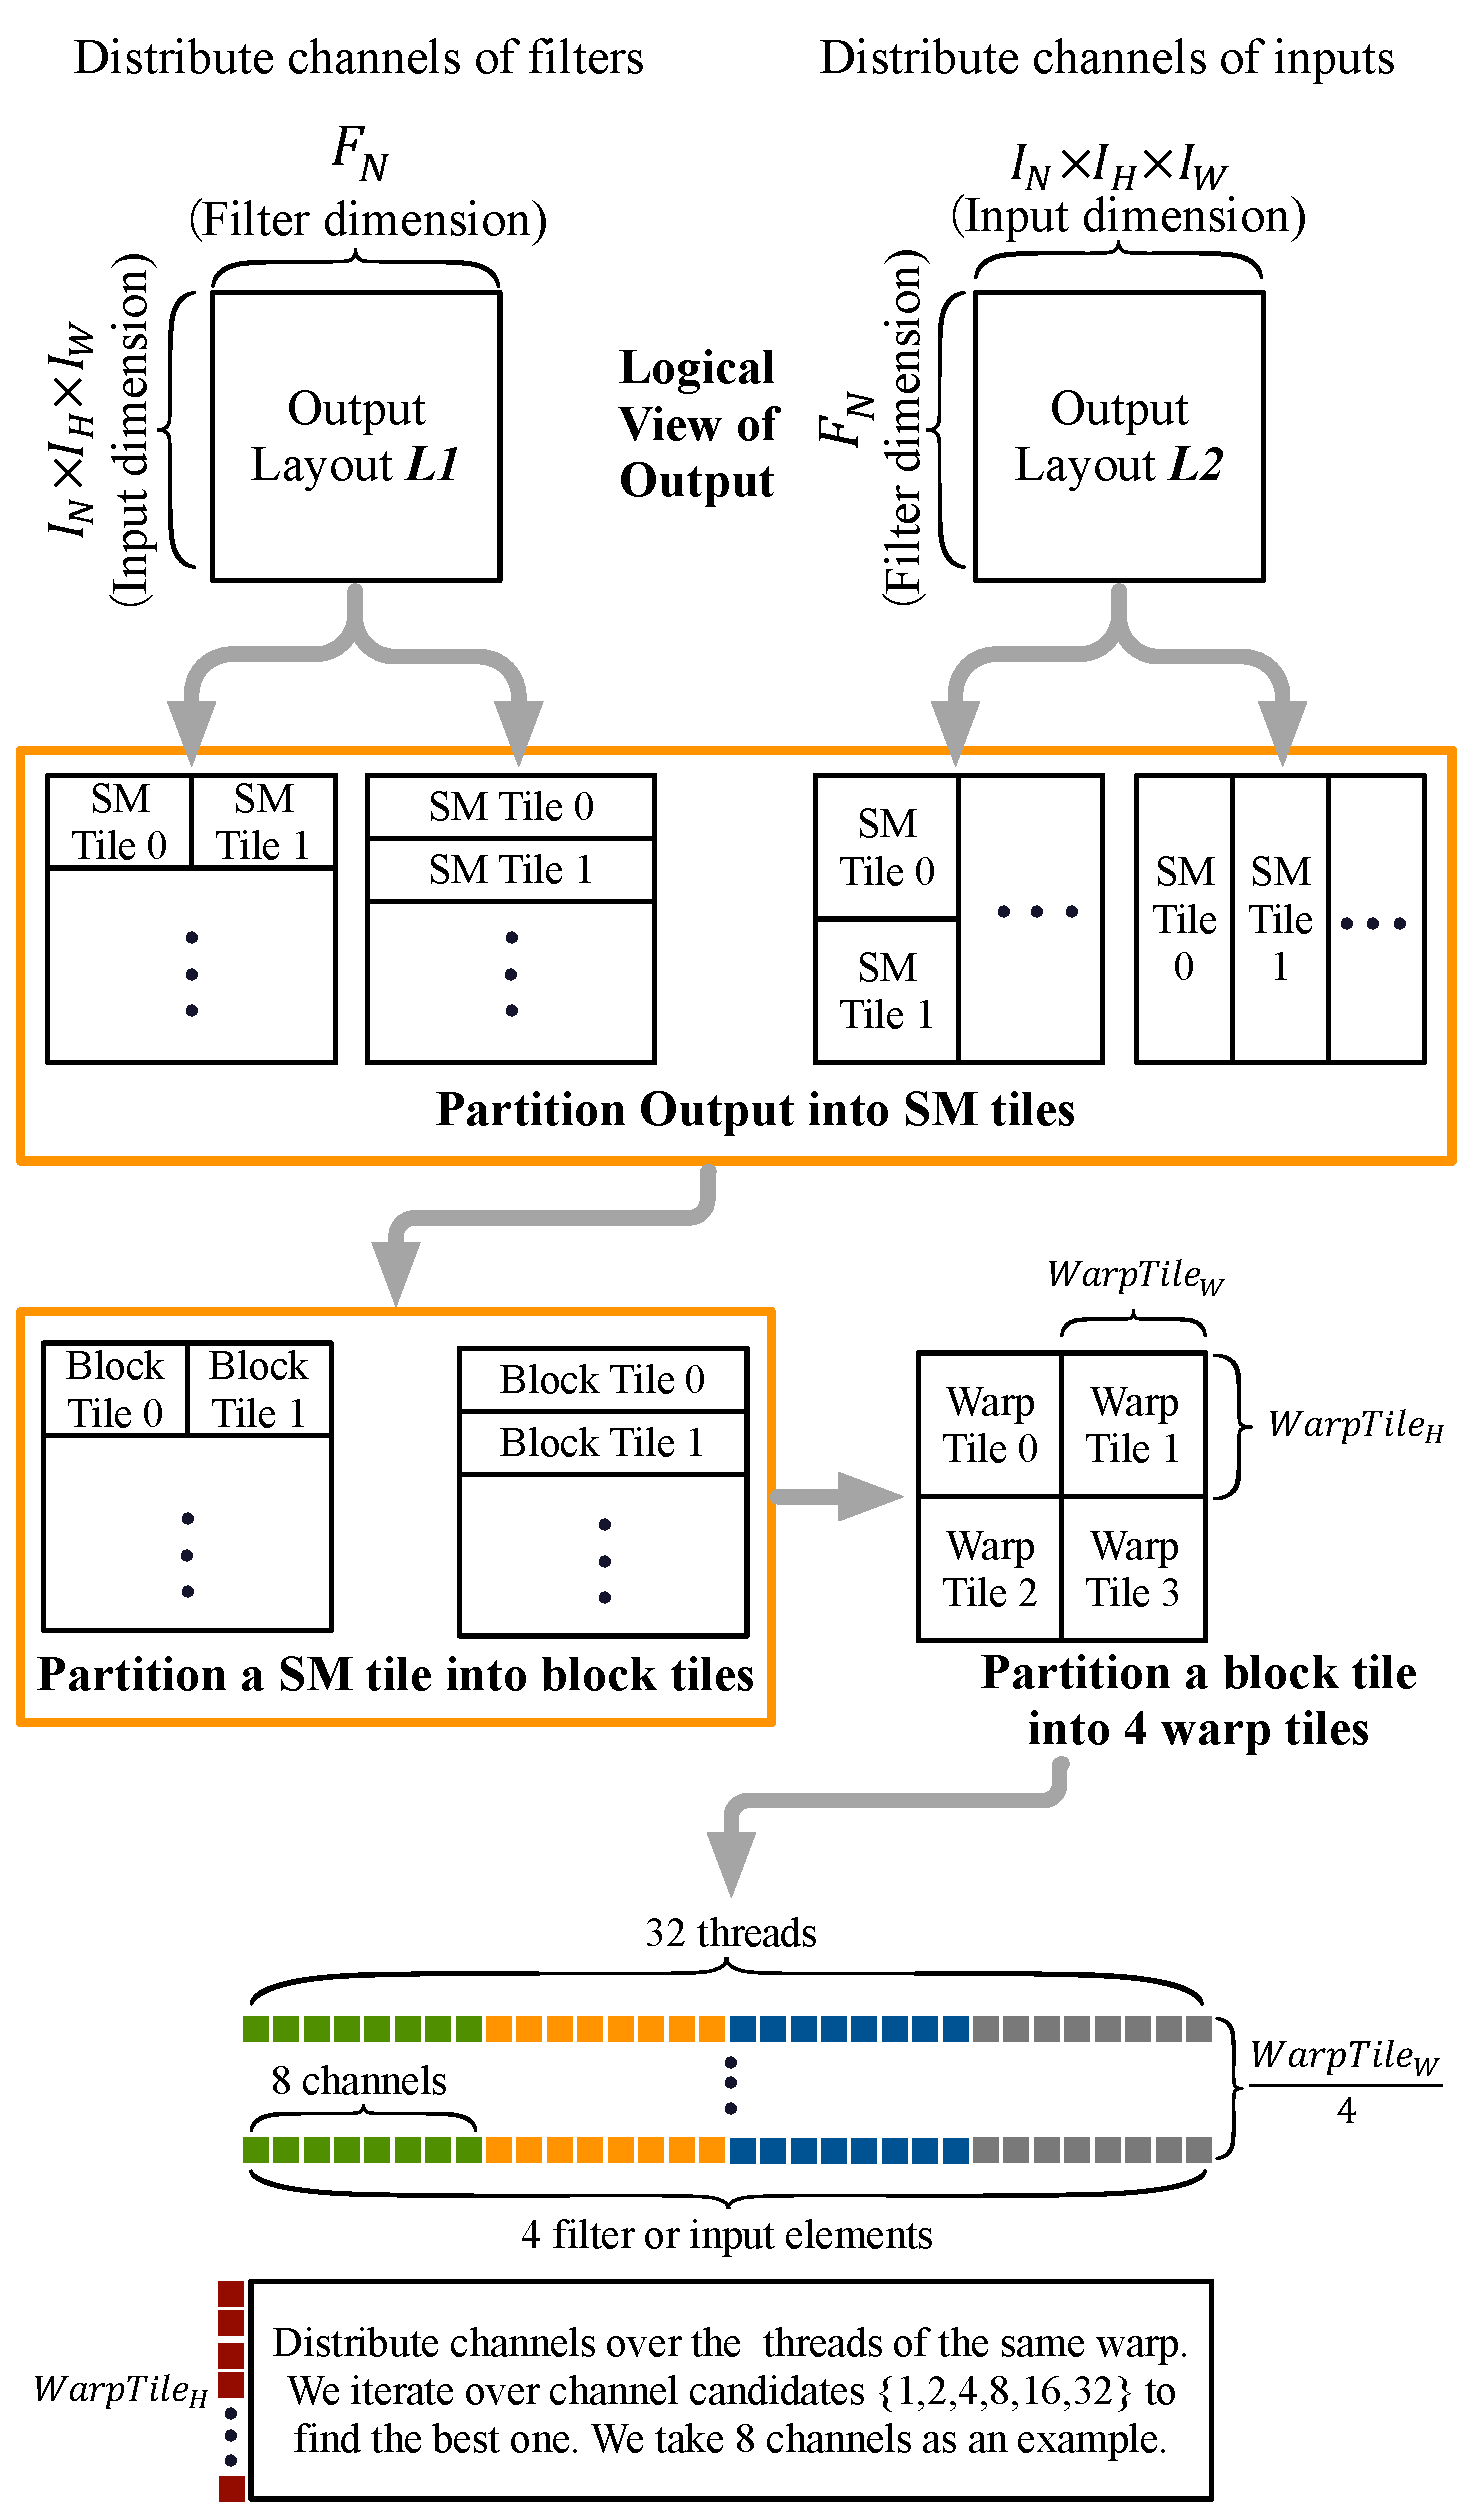
\includegraphics[width=0.95\textwidth,height=7cm]{./figure/pwworkflow.eps}
    \caption{Workflow of our dynamic block size method.} \label{fig:pwworkflow}
\end{figure*}
\begin{algorithm}[t!]
    \small
        \KwIn{$I$, $F$}
        \KwOut{$O$}
        $Warp_{num} \gets 4$, $Block_{num} \gets \{2,4\}$\;
        $C_{num} \gets \{1,2,4,8,16,32\}$\;
        \tcp{below codes are executed on CPU}
        Choose the layout and partition the output based on $F_N$\;
        \If{$I_N \times I_H \times I_W < 16 \times 14 \times 14$}{
            If use layout \textbf{\emph{L1}} (\textbf{\emph{L2}}), we set $Warp_H$ ($Warp_W$) $\gets$ \{2,3,4,5,6,7,8\}\;
        }
        \Else{
            If use layout \textbf{\emph{L1}} (\textbf{\emph{L2}}), we set $Warp_H$ ($Warp_W$) $\gets$ \{6,7,8,9,10,11,12\}\;
        }
        $preSM \gets MAX\_FLOAT$,$preD \gets MAX\_INT$\;
        \ForEach{combination of $Block_{num}$, $C_{num}$ and $Warp_H$ ($Warp_W$)}{
            \If{not satisfy constraints of Formula \ref{fo:limitr} and \ref{fo:limits}}{
                continue\;
            }
            Calculate $SM_{util}$ and $D$ with Formula \ref{fo:smutil} and \ref{fo:diff}\;
            \If{$preSM \geq 1$ and $SM_{util} \geq 1$ and both are close enough}{
                \If{$D < preD$}{
                    $preSM \gets min(preSM,SM_{util})$\;
                    $preD \gets D$, record the combination\;
                }
            }
            \ElseIf{$preSM \geq 1$ and $SM_{util} \geq 1$ and $SM_{util}<preSM$}{
                $preSM \gets SM_{util}$\;
                $preD \gets D$, record the combination\;
            }
            \ElseIf{$preSM <1$ and $SM_{util}<1$ and both are close enough}{
                \If{$D<preD$}{
                    $preSM \gets max(preSM,SM_{util})$\;
                    $preD \gets D$, record the combination\;
                }
            }
            \ElseIf{$preSMRl$ and $SM_{util}<1$ and $SM_{util}>preSM$}{
                $preSM \gets SM_{util}$,$preD \gets D$, record the combination\;
            }
            
        }
        Choose the proper kernel based on the recorded $Block_{num}$, $C_{num}$ and $Warp_H$.\;
        \tcp{below codes are executed on GPU}
        Each thread block loads $k\times C_{num}$ channels of the needed input and filter into shared memory array $sharedBuf1$\;
        $\_\_syncthreads()$\;
        \For{$iter \gets 0$ \KwTo $I_C$ By $2 \times k \times C_{num}$}{
            Load next $k \times C_{num}$ channels of input and filter into temporary registers\;
            Load current channels of input and filter from $sharedBuf1$ into registers\;
            Accumulate output elements $k$ times\;
            Write temporary registers into shared memory $sharedBuf2$\;
            $\_\_syncthreads()$\;
            Repeat above steps but swap $sharedBuf1$ and $sharedBuf2$\;
        }
        Use segmented parallel reduce to get the final output elements and write the result to $O$\;
        \caption{Pointwise Convolution Optimization}
        \label{algo:pwalgo}
\end{algorithm}

To guide the search for the optimal combination of $Block_{num}$, $C_{num}$ and $Warp_H$, we use two metrics named SM utilization ($SM_{util}$) and the difference between $Warp_H$ and $T_{num}$ ($D$).
Two metrics can be calculated as follows:
\begin{equation}\nonumber
    Block_{count}=\frac{F_N}{Block_W} \times \frac{I_N \times I_H \times I_W}{2 \times Warp_H}
\end{equation}
\begin{equation}
    SM_{util}=\frac{Block_{count}}{Block_{num}\times SM_{num}}
    \label{fo:smutil}
\end{equation}
\begin{equation}
    D = |Warp_H-T_{num}|
    \label{fo:diff}
\end{equation}
where $Block_{count}$ is the number of generated thread blocks, $SM_{num}$ is the number of SMs on a GPU. For RTX 2080Ti and AGX Xavier, $SM_{num}=48$ and $SM_{num}=8$ respectively.

We will demonstrate how to select the optimal combination based on both metrics in the next section.

\subsection{Putting Together}
The whole workflow is described in Algorithm \ref{algo:pwalgo}.
We first choose the layout of output and partition the output into block tiles based on $F_N$ (Line 3).
Second, we choose the candidate set for $Warp_H$ based on $I_N \times I_H \times I_W$ (Lines 4-7).
Then we iterate over all combinations of $Block_{num}$, $C_{num}$ and $Warp_H$ (Line 9), and keep the combinations that satisfy the constraints $Limit_R$ (Formula \ref{fo:limitr}) and $Limit_S$ (Formula \ref{fo:limits}).

Next, we calculate values of $SM_{util}$ (Formula \ref{fo:smutil}) and $D$ (Formula \ref{fo:diff}) for all satisfied combinations (Line 12) and select the optimal combination with following steps:
\begin{enumerate}[Step 1]
    \item If $SM_{util} \geq 1$ is true for all combinations, we select the combinations that possess the smallest and close to the smallest $SM_{util}$ (Lines 13, 17).
    The reason is that when $SM_{util} \geq 1$, all SMs are utilized, in which case we want to reduce the number of thread blocks to reduce the number of loads of shared filters or inputs between multiple thread blocks.
    \item If there exists combinations such that $SM_{util}<1$, we first collect these combinations. Then, among collected combinations, we select the ones that possess the biggest and close to the biggest $SM_{util}$ (Lines 20, 24).
    The reason is that when $SM_{util}<1$, there are idle SMs, in which case we want to increase $SM_{util}$ to fully utilize SMs. We do not want $SM_{util}$ to exceed 1 because that will incur more memory operations.
    \item Among candidate combinations selected in Step 1 and Step 2, we select the combination with the smallest value of $D$ (Line 14, 21) because we try to form $Warp_H$ and $T_{num}$ into a square shape to increase arithmetic intensity.
\end{enumerate}

Last, we choose the pointwise convolution kernel based on the selected combination of $Block_{num}$, $C_{num}$ and $Warp_H$ (Line 26). 
In this kernel, each thread block first loads $k \times C_{num}$ channels of corresponding inputs and filters into a shared memory array (Line 30). 
Then, each thread accumulates output elements $k$ times (Line 32). 
Meanwhile, the thread block loads the next $k \times C_{num}$ channels into another shared memory array (Line 31). 
We also use the double buffer method to increase the computational workload of each thread (Line 35).
The kernel repeats the process until all channels have been accumulated to output elements.
Finally, we use a warp level segmented parallel reduction to reduce results of different channels into the final result and write results to global memory (Line 36).  